%%%%%%%%%%%%%%%%%%%%%%%%%%%%%%%%%%%%%%%%%
% Beamer Presentation
% LaTeX Template
% Version 1.0 (10/11/12)
%
% This template has been downloaded from:
% http://www.LaTeXTemplates.com
%
% License:
% CC BY-NC-SA 3.0 (http://creativecommons.org/licenses/by-nc-sa/3.0/)
%
%%%%%%%%%%%%%%%%%%%%%%%%%%%%%%%%%%%%%%%%%

%----------------------------------------------------------------------------------------
%	PACKAGES AND THEMES
%----------------------------------------------------------------------------------------

\documentclass{beamer}

\mode<presentation> {

% The Beamer class comes with a number of default slide themes
% which change the colors and layouts of slides. Below this is a list
% of all the themes, uncomment each in turn to see what they look like.

%\usetheme{default}
%\usetheme{AnnArbor}
%\usetheme{Antibes}
%\usetheme{Bergen}
%\usetheme{Berkeley}
%\usetheme{Berlin}
%\usetheme{Boadilla}
%\usetheme{CambridgeUS}
%\usetheme{Copenhagen}
%\usetheme{Darmstadt}
%\usetheme{Dresden}
%\usetheme{Frankfurt}
%\usetheme{Goettingen}
%\usetheme{Hannover}
%\usetheme{Ilmenau}
%\usetheme{JuanLesPins}
%\usetheme{Luebeck}
\usetheme{Madrid}
%\usetheme{Malmoe}
%\usetheme{Marburg}
%\usetheme{Montpellier}
%\usetheme{PaloAlto}
%\usetheme{Pittsburgh}
%\usetheme{Rochester}
%\usetheme{Singapore}
%\usetheme{Szeged}
%\usetheme{Warsaw}

% As well as themes, the Beamer class has a number of color themes
% for any slide theme. Uncomment each of these in turn to see how it
% changes the colors of your current slide theme.

%\usecolortheme{albatross}
%\usecolortheme{beaver}
%\usecolortheme{beetle}
%\usecolortheme{crane}
%\usecolortheme{dolphin}
%\usecolortheme{dove}
%\usecolortheme{fly}
%\usecolortheme{lily}
%\usecolortheme{orchid}
%\usecolortheme{rose}
%\usecolortheme{seagull}
%\usecolortheme{seahorse}
%\usecolortheme{whale}
%\usecolortheme{wolverine}

%\setbeamertemplate{footline} % To remove the footer line in all slides uncomment this line
%\setbeamertemplate{footline}[page number] % To replace the footer line in all slides with a simple slide count uncomment this line

%\setbeamertemplate{navigation symbols}{} % To remove the navigation symbols from the bottom of all slides uncomment this line
}

\usepackage{graphicx} % Allows including images
\usepackage{booktabs} % Allows the use of \toprule, \midrule and \bottomrule in tables

%----------------------------------------------------------------------------------------
%	TITLE PAGE
%----------------------------------------------------------------------------------------

\title[Comparison of classifiers]{A comparison Of classifiers for oil spill detection} % The short title appears at the bottom of every slide, the full title is only on the title page

\institute[TUDelft] % Your institution as it will appear on the bottom of every slide, may be shorthand to save space
{
Delft University of Technology \\ % Your institution for the title page
\medskip
%\textit{john@smith.com} % Your email address
}
\date{\today} % Date, can be changed to a custom date
\author{A.S.Y.Chiu\\ T.P.van Helden\\S.S.Jahanshahi} % Your name

\begin{document}

\begin{frame}
\titlepage % Print the title page as the first slide
\end{frame}

\begin{frame}
\frametitle{Overview} % Table of contents slide, comment this block out to remove it
\begin{enumerate}
	\item Introduction
	\item SAR preprocessing
	\item Features
	\item Summary of Classifiers 
	\begin{itemize}
		\item Support Vector Machine
		\item Multi Layer Perceptron
		\item Descision Trees
		
	\end{itemize}
	\item Compariosn of Classifiers
\end{enumerate}

%\tableofcontents % Throughout your presentation, if you choose to use \section{} and \subsection{} commands, these will automatically be printed on this slide as an overview of your presentation
\end{frame}

%----------------------------------------------------------------------------------------
%	PRESENTATION SLIDES
%----------------------------------------------------------------------------------------

%------------------------------------------------
%\section{First Section} % Sections can be created in order to organize your presentation into discrete blocks, all sections and subsections are automatically printed in the table of contents as an overview of the talk
%------------------------------------------------

%\subsection{Subsection Example} % A subsection can be created just before a set of slides with a common theme to further break down your presentation into chunks

\begin{frame}
\frametitle{Introduction}
\begin{minipage}[h]{0.33\textwidth}
\begin{figure}
	\centering
    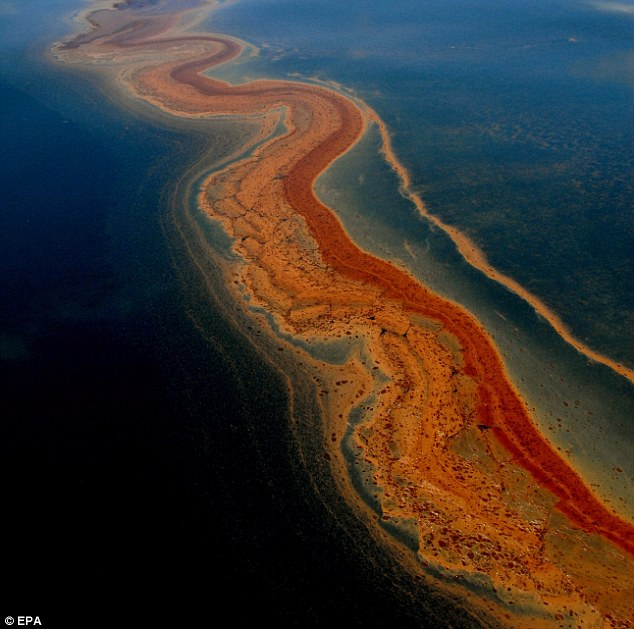
\includegraphics[width=60mm,scale=1]{./img/mex.jpg}
\end{figure}
\end{minipage}

\begin{minipage}[h]{0.33\textwidth}
\begin{itemize}
	\item What is an oil spill?
	\item Why is of importance to detect oil spill? %enviornmental pollution,BP pais 27 bilion for cleanup in gulf of mexico
	\item How to detect oil spills? %SAR image, difference of Oil spill & lookalike
	
	
\end{itemize}
\end{minipage}

\end{frame}

\begin{frame}
\frametitle{General oil spill detection approach}
\begin{figure}
	\centering
    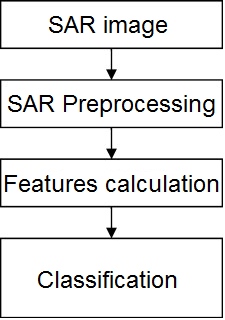
\includegraphics[width=40mm,scale=1]{./img/basicsteps.png}
\end{figure}



\end{frame}
%------------------------------------------------
\begin{frame}
\frametitle{SAR image}
\begin{itemize}
	\item Has high resolution
	\item Can monitor ocean 24 hours a day
	\item Covers large area 

\end{itemize}
\end{frame}
%----------------
\begin{frame}
\frametitle{SAR preprocessing}
\begin{figure}
	\centering
    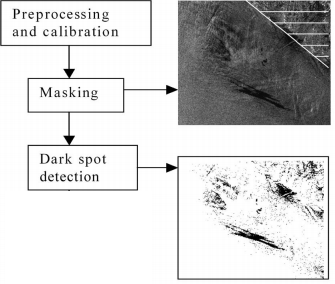
\includegraphics[width=60mm,scale=1]{./img/preprocessing_diagram.png}
\end{figure}
\end{frame}

%------------------------------------------------

\begin{frame}
\frametitle{Features}
\begin{itemize}
	\item What is features?
	\item Type of features \begin{itemize}
					\item Geometrical %area,perimeter, complexity
					\item Physical %mean, max backscatter value
					\item Texture %mean,contrast
					\item Contextual  %distance between dark spots
					\end{itemize}
				
\end{itemize}

\end{frame}

%------------------------------------------------

\begin{frame}
\frametitle{Feature Selection}
\begin{itemize}
	\item Choosing features
	\item Overfitting 
	\item Curse of dimensionality
\end{itemize}
\begin{figure}
	\centering
    \includegraphics[width=60mm,scale=1.5]{./img/overfit.png}
\end{figure}
\end{frame}
%-----------------------------------------

\begin{frame}
\frametitle{Supervised learning}

\begin{figure}
	\centering
    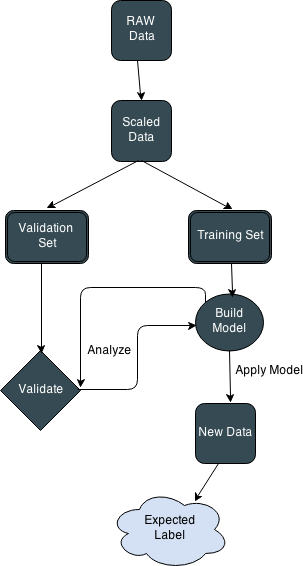
\includegraphics[width=40mm,scale=1]{./img/SL.png}
\end{figure}

\end{frame}

%------------------------------------------------

\begin{frame}
\frametitle{Support vector machines}
\begin{figure}
	\centering
    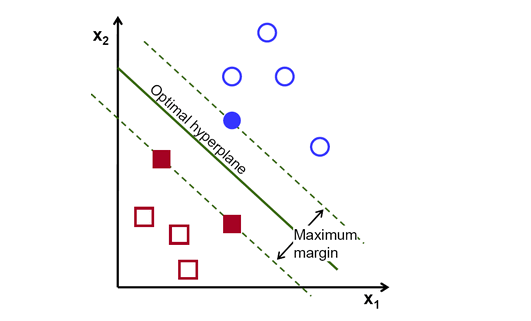
\includegraphics[width=90mm,scale=1]{./img/SVM.png}
\end{figure}

\end{frame}

%------------------------------------------------

\begin{frame} % Need to use the fragile option when verbatim is used in the slide
\frametitle{Decision Tree}
\begin{figure}
	\centering
    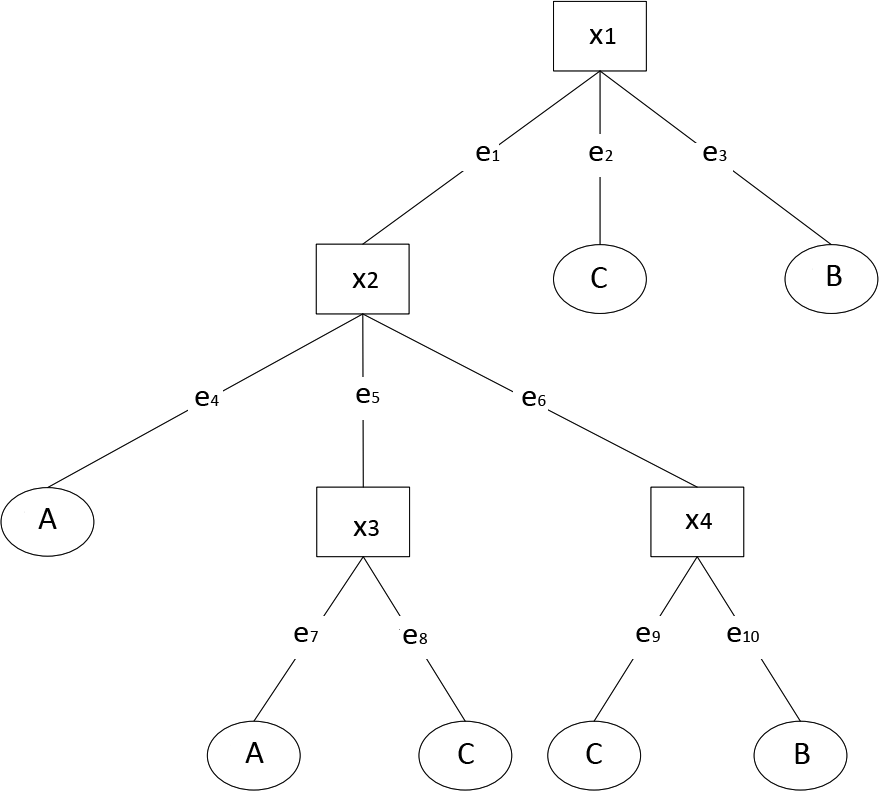
\includegraphics[width=70mm,scale=1]{./img/decisiontree.png}
\end{figure}

\end{frame}

%------------------------------------------------
\begin{frame} % Need to use the fragile option when verbatim is used in the slide
\frametitle{Perceptron}
\begin{figure}
	\centering
    
\includegraphics[width=90mm,scale=1]{./img/perceptron.png}
\end{figure}

\end{frame}
\begin{frame}
\frametitle{Multi layer perceptrons}
\begin{figure}
	\centering
    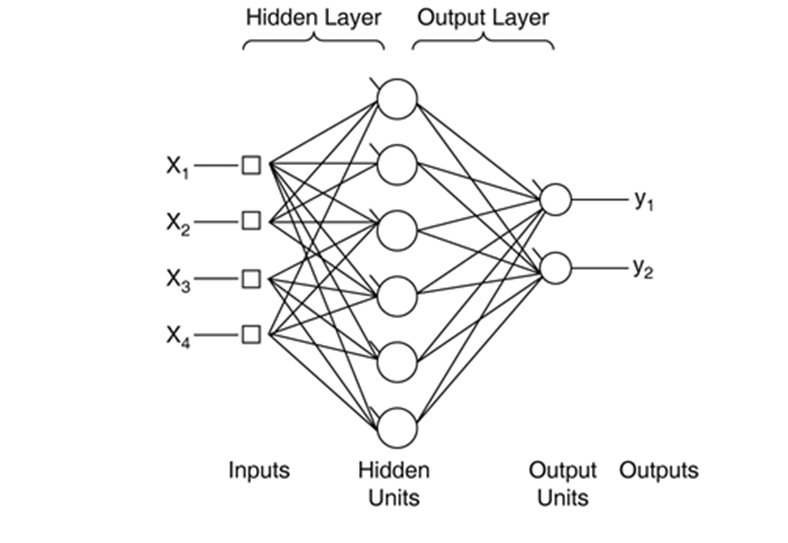
\includegraphics[width=90mm,scale=1]{./img/MLP.jpg}
\end{figure}
\end{frame}


%------------------------------------------------

\begin{frame}
\frametitle{Comparison of classifiers}
\begin{itemize}
	\item Free lunch theorem
	\item Criteria for comparison %accuracy performance
	 
\end{itemize}
\end{frame}

%------------------------------------------------



%------------------------------------------------

\begin{frame}
\Huge{\centerline{The End}}
\end{frame}

%----------------------------------------------------------------------------------------

\end{document} 